\documentclass[a4paper]{article}

\usepackage[french]{babel}
\usepackage[utf8]{inputenc}
\usepackage{graphicx}

\begin{document}

\title{Rapport préliminaire du projet}
\author{Stéphane \textsc{Maniaci} \\
	Baptiste \textsc{Saleil} \\
	\textbf{tutoré par :} Abdelkader \textsc{Gouaich}}
\date\today

\maketitle

\tableofcontents

\clearpage

\part{Présentation du projet}

L'objectif du projet est de créer une série de mini-jeux basés sur le mouvements pour \
permettre à des personnes victimes d'un AVC de pouvoir travailler leur motricité d'une façon ludique.\
Ils auront pour cela une clé USB à leur disposition sur laquelle ils pourront directement \
démarrer les jeux et s'entraîner avec un contrôleur sans-fil (\textit{i.e} une Wiimote) . \
\\ \\
Le programme doit être capable de tracer leur mouvements et leur progression\
(système de score) afin de pouvoir exploiter les résultats de cette évolution si\
ils s'avèrent utiles aux médecins qui les prennent en charge. On envisage notamment\
de remonter les données sur un serveur principal dans le centre du patient.
\\ \\
Ce projet est proposé et tutoré par Mr. Abdelkader \textsc{Gouaich}.

\clearpage

\part{Inspirations}

Les jeux seront divisés en catégories pour permettre une diversité ludique avec quand même \
une progression globale pour conserver une certaine linéarité malgré les différents \
types de jeu.

\section*{Jeu de tir à la première personne} 
Le but du jeu est de tirer sur des objets volants, d'un point de tir statique. Inspiré d'un jeu de \textit{Wii Play},\
nous développerons le \textit{game design} une fois que l'on aura obtenu un prototype fonctionnel.
\\
\begin{figure}[h!]
\begin{center}\includegraphics[width=7cm]{img/wii.ps}\end{center}
\caption{Capture du jeu de tir sur Wii Play}
\end{figure}

\section*{Jeu de dessin}
Inspirée par le jeu \textit{Rayman contre les lapins crétins} sur Wii, le but\
est de surligner à l'écran des motifs indiqués par le jeu. Là encore, on attendra \
d'avoir un prototype fonctionnel pour décider les détails artistiques. \

\begin{figure}[h!]
\begin{center}\includegraphics[width=6cm]{img/wiidessin.ps}\end{center}
\caption{Capture du jeu de tir sur Wii Play}
\end{figure}

\clearpage

\part{Spécifications techniques}

\section{Langage de programmation}
Comme proposé dans l'énoncé du projet, nous utiliserons \bsc{C++} et la librairie graphique\
\bsc{Qt} dans sa version embarquée, cette dernière permettant des économies de ressources \
et une portabilité maximale.
Google Code offre une gestion du code avec Subversion, qui est un \
système de révision du code, mais nous utiliserons Git à la place, un système plus récent \
(développé pour le noyau Linux) qui permet de travailler sur le projet en hors-ligne.

\section{Infrastructure de développement}
Nous allons utiliser au maximum la plateforme Google pour mener à bien notre projet :
\begin{itemize}
\item{\textbf{Google Code} pour l'hébergement du code, bugtracking, wiki ;}
\item{\textbf{Google Documents} pour le partage de notes et documents;}
\item{\textbf{Google Mail} pour la communication et le chat entre développeurs;}
\item{\textbf{Google Groups} si nous en venons à utiliser une liste de discussions.}
\end{itemize}

\section{Élements du jeu}
Le patient lancera le jeu depuis sa clé USB, et arrivera sur un menu principal simple \
et concis, pour lui permettre d'accéder aux jeux triés par catégorie. \
Il nous faudra donc coder dans un premier temps un \textbf{moteur central} capable de gérer \
\textbf{l'affichage 2D, la journalisation}, et qui fournisse une \textbf{architecture de base} \
avec les classes de base sur lesquelles seront construites les jeux.
L'affichage doit \textbf{se passer d'un serveur X} (par économie de ressources), nous écrirons donc directement \
sur le framebuffer grâce à Qt Embedded. 
La journalisation se fera dans des fichiers clairs (plain text), nous n'avons pas encore\
défini sous quelle forme, ce sera décrit dans le premier compte-rendu. Les diagrammes fourni \
par l'analyse UML apporteront plus de précision dans quelques semaines.

\clearpage

\part{Feuille de route}

Nous avons défini dans un premier temps les étapes nécessaires à la réalisation du projet\
mais les dates arrêtés seront décidées dans le prochain rapport. Voici donc la liste\
des objectifs principaux à atteindre.

\begin{enumerate}
\item{Définition du projet et des moyens à mettre en \oe uvre ;}
\item{Analyse UML du projet ;}
\item{Prise en main de \bsc{Qt} et \bsc{C++}}
\item{Mise en place d'un environnement de développement ;}
\item{Réalisation d'un premier jeu fonctionnel dont sera dégagé le moteur ;}
\item{Optimisation et finalisation du moteur ;}
\item{Réalisation des jeux du projet ;}
\item{Optimisation, finalisation et documentation du projet ;}
\item{Champagne !}
\end{enumerate}

\end{document}
